% Dit werk is gelicenseerd onder de licentie Creative Commons Naamsvermelding-GelijkDelen 4.0 Internationaal. Ga naar http://creativecommons.org/licenses/by-sa/4.0/ om een kopie van de licentie te kunnen lezen.
\chapter{Leidingstelsels}
\label{sec:Leidingstelsels}
%%%%%%%%%%%%%%%%%%%%%%%%%%%%%%%%%%%%%%%%%%%%%%%%%%%%%%%%%%%%%%%%%%%%%%%%%%%%%%%%%%%%%%
\begin{toepassing}[*]
	\label{warmtewisselaar}
Een sectie van een warmtewisselaar bestaat uit 100 parallelle kanalen met een cirkelvormige doorsnede, een binnendiameter van $10 \unit{mm}$ en lengte $400 \unit{mm}$ en een ruwheid van $0.005 \unit{mm}$. Door deze warmtewissellaar stroomt lucht ($\rho=1.2 \unit{kg/m^3}$, $\nu=15 \unit{mm^2/s}$) met een debiet van $360 \unit{m^3/h}$.
		
Bepaal de drukval over de warmtewissellaar, verwaarloos lokale verliezen aan in en uitlaat.	
\end{toepassing}
\begin{antwoord}{\ref{warmtewisselaar}}
	$\Delta p = 128 \unit{Pa}$
\end{antwoord}
%%%%%%%%%%%%%%%%%%%%%%%%%%%%%%%%%%%%%%%%%%%%%%%%%%%%%%%%%%%%%%%%%%%%%%%%%%%%%%%%%%%%%%
\begin{toepassing}[*]
	\label{serie parallel}
Een leidingstelsel bestaat uit 4 leidingen A-D zoals aangegeven op onderstaande figuur. Leiding A heeft lengte $2000 \unit{m}$ en diameter $0.200 \unit{m}$, leiding B heeft lengte $3000 \unit{m}$ en diameter $.150 \unit{m}$, leiding C heeft lengte $2000 \unit{m}$ en diameter $0.100 \unit{m}$ en , leiding D heeft lengte $1000 \unit{m}$ en diameter $0.180 \unit{m}$. Alle leidingen hebben een ruwheid van $0.5 \unit{mm}$. Doorheen het stelsel stroomt water ($\rho=1000 \unit{kg/m^3}$, $\nu=1 \unit{mm^2/s}$) met een debiet van $200 \unit{m^3/h}$.

Bepaal de drukval over het leidingstelsel indien beide uiteindes zich op dezelfde hoogte bevinden. Verliezen in de splitsing en samenvoeging mogen verwaarloosd worden.

	\centering
	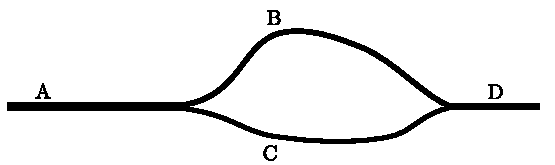
\includegraphics{fig/leidingstelsels/serie_parallel}
\end{toepassing}
\begin{antwoord}{\ref{serie parallel}}
	$\Delta p = 2080 \unit{kPa}$
\end{antwoord}
%%%%%%%%%%%%%%%%%%%%%%%%%%%%%%%%%%%%%%%%%%%%%%%%%%%%%%%%%%%%%%%%%%%%%%%%%%%%%%%%%%%%%%
\begin{toepassing}
	\label{geperforeerde leiding hoogteverschil}
Een hoofdleiding met een diameter van $675 \unit{mm}$ loopt horizontaal over $1500 \unit{m}$ en splitst dan in 2 dezelfde leidingen $d=450 \unit{mm}$ en $l=3000 \unit{m}$. Beide leidingen zijn open op het einde en komen op de zelfde eindhoogte uit, maar één van de twee leidingen heeft ook openingen in de zijwand. Hierdoor gaat de helft van het water afgevoerd worden over de totale lengte van de leiding.

Als de wrijvingsfactor 0.024 is voor alle leidingen en het debiet is $0.28 \unit{m^3/s}$ water ($\rho=1000 \unit{kg/m^3}$, $\nu=1 \unit{mm^2/s}$) in de hoofdleiding, bereken dan het hoogteverschil tussen het vloeistof oppervlak en de plaats waar de vloeistof in de atmosfeer komt. Men mag de vertragingsverliezen verwaarlozen.
\end{toepassing}
\begin{antwoord}{\ref{geperforeerde leiding hoogteverschil}}
	$\Delta h = 6.42 \unit{m}$
\end{antwoord}
%%%%%%%%%%%%%%%%%%%%%%%%%%%%%%%%%%%%%%%%%%%%%%%%%%%%%%%%%%%%%%%%%%%%%%%%%%%%%%%%%%%%%%
\begin{toepassing}
	\label{parallelle leidingen}
Twee open water reservoirs ($\rho=1000 \unit{kg/m^3}$, $\nu=1 \unit{mm^2/s}$) zijn met elkaar verbonden door 3 afzonderlijke leidingen met diameters $d$, $2d$, $3d$. De leidingen hebben allen dezelfde lengte.
		
Veronderstel dat de wrijvingsfactoren gelijk zijn, wat zal dan het volumedebiet doorheen de twee grootste leidingen zijn als het debiet door de kleinste leiding gelijk is aan $0.03 \unit{m^3/s}$? 
\end{toepassing}
\begin{antwoord}{\ref{parallelle leidingen}}
	$\dot{V}_\mathrm{B} = 0.17 \unit{m^3/s}$, $\dot{V}_\mathrm{C} = 0.47 \unit{m^3/s}$
\end{antwoord}
%%%%%%%%%%%%%%%%%%%%%%%%%%%%%%%%%%%%%%%%%%%%%%%%%%%%%%%%%%%%%%%%%%%%%%%%%%%%%%%%%%%%%%
\begin{toepassing}[*]
	\label{turbulent laminair}
	Twee open water reservoirs ($\rho=1000 \unit{kg/m^3}$, $\nu=1 \unit{mm^2/s}$) zijn met elkaar verbonden door een leiding met diameter $100 \unit{mm}$ en lengte $200 \unit{m}$ en een leiding met diameter $10 \unit{mm}$ en lengte $20 \unit{m}$. De ruwheid van beide leidingen is $0.01 \unit{mm}$.
	
Bepaal het debiet door elk van de leidingen indien het hoogteverschil tussen de 2 water niveau's $0.1 \unit{m}$ bedraagt en je de lokale verliezen aan in en uitlaat mag verwaarlozen.
\end{toepassing}
\begin{antwoord}{\ref{turbulent laminair}}
	$\dot{V}_\mathrm{A} = 88 \unit{l/min}$, $\dot{V}_\mathrm{B} = 0.72 \unit{l/min}$
\end{antwoord}
%%%%%%%%%%%%%%%%%%%%%%%%%%%%%%%%%%%%%%%%%%%%%%%%%%%%%%%%%%%%%%%%%%%%%%%%%%%%%%%%%%%%%%
\begin{toepassing}
	\label{gesplitste gelijke leidingen}
Twee open water reservoirs ($\rho=1000 \unit{kg/m^3}$, $\nu=1 \unit{mm^2/s}$), waarvan het verschil tussen de twee vloeistofniveaus $6 \unit{m}$ is, zijn door een leiding met elkaar verbonden. De leiding ($d=600 \unit{mm}$) vertrekt in het reservoir met het hoogste waterniveau. Na $3000 \unit{m}$ splitst de leiding in 2 leidingen ($d=300 \unit{mm}$) van elk $3000 \unit{m}$ lang. Deze leidingen komen beide aan in het tweede reservoir. 
		
Als de wrijvingsfactor gelijk is aan $0.04$ bepaal dan het totale volumedebiet. 
\end{toepassing}
\begin{antwoord}{\ref{gesplitste gelijke leidingen}}
	$\dot{V} = 0.0723 \unit{m^3/s}$
\end{antwoord}
%%%%%%%%%%%%%%%%%%%%%%%%%%%%%%%%%%%%%%%%%%%%%%%%%%%%%%%%%%%%%%%%%%%%%%%%%%%%%%%%%%%%%%
\begin{toepassing}[*]
	\label{gesplitste ongelijke leidingen}
Een open water reservoirs ($\rho=1000 \unit{kg/m^3}$, $\nu=1 \unit{mm^2/s}$), stroomt leeg via een leiding met een diameter van $200 \unit{mm}$. Na $20 \unit{m}$ splitst de leiding in 2 leidingen waarvan de eerste een diameter van $120 \unit{mm}$ heeft en de tweede een diameter van $80 \unit{mm}$. Na $10 \unit{m}$ stromen beide leidingen vrij uit in de atmosfeer op een hoogte $10 \unit{m}$ onder het waterniveau in het reservoir. Alle leidingen hebben een ruwheid van $0.01 \unit{mm}$.

Bepaal het debiet in elke leiding, verwaarloos lokale verliezen.
\end{toepassing}
\begin{antwoord}{\ref{gesplitste ongelijke leidingen}}
	$\dot{V}_\mathrm{A} = 0.151 \unit{m^3/s}$, $\dot{V}_\mathrm{B} = 0.112 \unit{m^3/s}$,\\
	$\dot{V}_\mathrm{C} = 0.039 \unit{m^3/s}$
\end{antwoord}
%%%%%%%%%%%%%%%%%%%%%%%%%%%%%%%%%%%%%%%%%%%%%%%%%%%%%%%%%%%%%%%%%%%%%%%%%%%%%%%%%%%%%%
\begin{toepassing}
	\label{geperforeerde leiding debiet}
Een open water reservoir ($\rho=1000 \unit{kg/m^3}$, $\nu=1 \unit{mm^2/s}$) voedt een leiding van $300 \unit{m}$ lang, diameter $200 \unit{mm}$. Deze leiding splitst in 2 gelijke leidingen $150 \unit{mm}$ in diameter en $150 \unit{m}$ lang. Beide leidingen zijn open op het einde en bevinden zich beide op een hoogte van $15 \unit{m}$ onder het vloeistofoppervlak van het reservoir. Eén leiding heeft een uniforme afvoer langs de zijwand en verliest over de volledige lengte de helft van de hoeveelheid water door die leiding. De wrijvingsfactor is $0.024$ voor beide leidingen. Alle lokale verliezen mogen verwaarloosd worden.
		
Bereken het volumedebiet van de twee leidingen afzonderlijk. 
\end{toepassing}
\begin{antwoord}{\ref{geperforeerde leiding debiet}}
	$\dot{V}_\mathrm{B} = 0.034 \unit{m^3/s}$, $\dot{V}_\mathrm{C} = 0.045 \unit{m^3/s}$
\end{antwoord}
%%%%%%%%%%%%%%%%%%%%%%%%%%%%%%%%%%%%%%%%%%%%%%%%%%%%%%%%%%%%%%%%%%%%%%%%%%%%%%%%%%%%%%
\begin{toepassing}
	\label{3uitlaten}
Een ventilatieleiding met diameter $300 \unit{mm}$ en ruwheid $1 \unit{mm}$ heeft 3 regelbare uitlaten op onderling gelijke afstand van $12.0 \unit{m}$. De ventielen moeten zo geregeld worden dat door elke uitlaat hetzelfde debiet stroomt. $\rho = 1.22 \unit{kg/m^3}$, $\nu = 15 \unit{mm^2/s}$.
	
Bepaal het ladingsverlies dat moet ingesteld worden aan de eerste twee uitlaten indien er vlak voor de eerste uitlaat een statische overdruk heerst van $50 \unit{Pa}$ en de laatste uitlaat een ladingsverlies van $5.00 \unit{m}$ veroorzaakt.

	\centering
	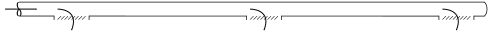
\includegraphics{fig/leidingstelsels/3uitlaten}
\end{toepassing}
\begin{antwoord}{\ref{3uitlaten}}
	$h_\mathrm{L,1} = 6.98 \unit{m}$, $h_\mathrm{L,2} = 5.41 \unit{m}$
\end{antwoord}
%%%%%%%%%%%%%%%%%%%%%%%%%%%%%%%%%%%%%%%%%%%%%%%%%%%%%%%%%%%%%%%%%%%%%%%%%%%%%%%%%%%%%%
\begin{toepassing}[*]
	\label{grondwarmtewisselaar}
Een grondwarmtewisselaar bestaat uit 2 parallelle boringen van elk $80 \unit{m}$ diepte. De twee boringen liggen $60 \unit{m}$ uit elkaar. Het volledige systeem is opgebouwd uit leidingen met een binnendiameter van $37 \unit{mm}$ en een ruwheid van $0.015 \unit{mm}$. Door de leidingen stroomt een anti-vries oplossing met een dichtheid van $1130 \unit{kg/m^3}$ en een viscositeit van $1.463 \unit{mPa\ s}$.
	
Bepaal de het debiet door elk van de boringen indien in de hoofdleiding een debiet van $50 \unit{l/min}$ stroomt.

	\centering	
	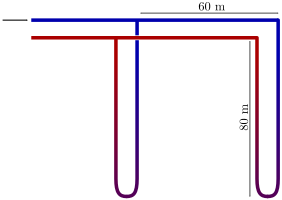
\includegraphics{fig/leidingstelsels/grondwarmtewisselaar}
\end{toepassing}
\begin{antwoord}{\ref{grondwarmtewisselaar}}
	$\dot{V}_\mathrm{A} = 29.0 \unit{l/min}$, $\dot{V}_\mathrm{B} = 21.0 \unit{l/min}$
\end{antwoord}
%%%%%%%%%%%%%%%%%%%%%%%%%%%%%%%%%%%%%%%%%%%%%%%%%%%%%%%%%%%%%%%%%%%%%%%%%%%%%%%%%%%%%%
\begin{toepassing}[*]
	\label{3reservoirs}
Drie open water reservoirs ($\rho=1000 \unit{kg/m^3}$, $\nu=1 \unit{mm^2/s}$) zijn verbonden zoals op onderstaande afbeelding. De wrijvingsfactor van de drie leidingen is $0.032$. In en uitstroom verliezen worden verwaarloosd.
		
Bepaal het debiet in alle drie de leidingen en de overdruk in het knooppunt.
		
	\centering
	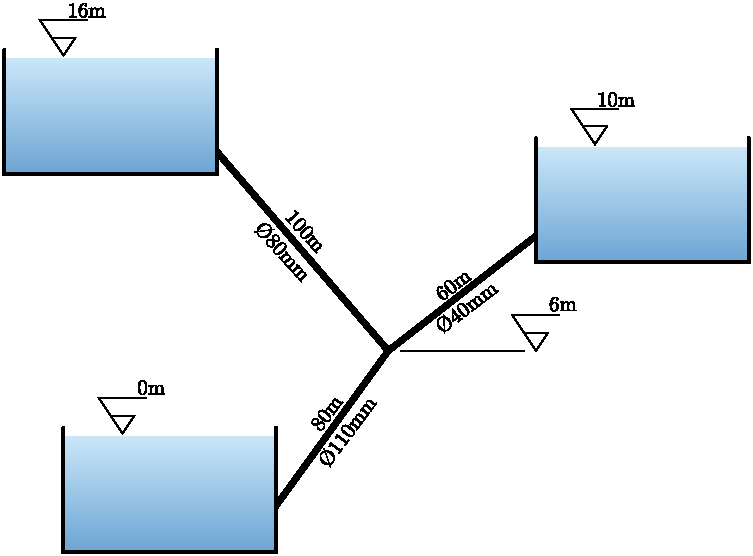
\includegraphics{fig/leidingstelsels/3reservoirs}
\end{toepassing}
\begin{antwoord}{\ref{3reservoirs}}
		$\dot{V}_\mathrm{A} = 764 \unit{l/min}$, $\dot{V}_\mathrm{B} = 128 \unit{l/min}$,\\
		$\dot{V}_\mathrm{C} = 893 \unit{l/min}$, $p=-31.6 \unit{kPa}$
\end{antwoord}
%%%%%%%%%%%%%%%%%%%%%%%%%%%%%%%%%%%%%%%%%%%%%%%%%%%%%%%%%%%%%%%%%%%%%%%%%%%%%%%%%%%%%%
\section*{Antwoorden}
	\begin{multicols}{2}
		\includecollection{antwoorden}
	\end{multicols}